\documentclass[12pt, french]{article}

\usepackage{fancyhdr, fancybox, lastpage}
\usepackage[most]{tcolorbox}
\usepackage[a4paper, margin={0.3in, .75in}]{geometry}
\usepackage{wrapfig}
\pagestyle{fancy}
\renewcommand\headrulewidth{1pt}
\renewcommand\footrulewidth{1pt}
\fancyhf{}
\rhead{ \em{Zakaria Haouzan}}
\lhead[C]{\em{2ème année baccalauréat Sciences Physiques}}
\chead[C]{}
\rfoot[C]{}
\lfoot[R]{}
\cfoot[]{\em{Page \thepage / \pageref{LastPage}}}


\newtcolorbox{Box2}[2][]{
                lower separated=false,
                colback=white,
colframe=white!20!black,fonttitle=\bfseries,
colbacktitle=white!30!gray,
coltitle=black,
enhanced,
attach boxed title to top left={yshift=-0.1in,xshift=0.15in},
title=#2,#1}


\begin{document}
\begin{center}
   \shadowbox {\bf{ Décroissance radioactive  }}
\end{center}

\vspace{-0.2cm}
%%_________________________Exercice ! :"_________________________Exercice
   \begin{Box2}{Exercice 1 :  Le polonium 210}
	   Le polonium 210 $_{84}^{210}Po$ est radioactif $\alpha$, sa désintégration conduit à la formation d’un isotope de plomb $_Z^APb$.La demi-vie du polonium $_{84}^{210}Po$ est $t_{1/2}=138jours$ 
	   \begin{enumerate}
		   \item Ecrire l’équation de désintégration de $_{84}^{210}Po$.
		   \item Calculer la constante radioactive de $_{84}^{210}Po$.
		   \item Sachant que l’activité initiale de l’échantillon de polonium 210 est $a_0 = 10^{10}Bq$.Calculer le nombre de
noyaux radioactifs $N_0$ dans l’échantillon à l’instant initial.
\item Déterminer la durée nécessaire pour que l’activité de l’échantillon soit égale à $a_0/4$.
\item Donner la relation entre $a_0$ et a(t) : l’activité de l’échantillon à un instant t

\item Exprimer la décroissance relative de l’activité $r=\frac{a_0 - a(t)}{a_0}$ en fonction de t1/2. Puis calculer r pour t=1jour.

\item Combien de temps faut-il attendre pour que $99,9\%$ d’une masse donnée de strontium 90 $(_{90}^{38}Sr)$ ait disparu ? On donne la demi-vie du strontium 90 est de 28ans
	   \end{enumerate}


   \end{Box2}


%%_________________________Exercice !2 :"_________________________Exercice
\begin{Box2}{Exercice 2 :isotopes radioactifs de l’iode }
%\begin{wrapfigure}{r}{0.22\textwidth}
  %\begin{center}
	  %\vspace{-0.6cm}
	%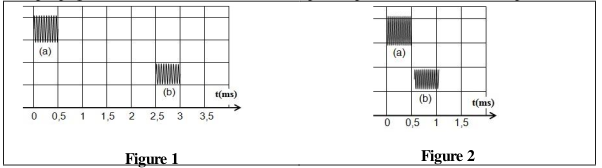
\includegraphics[width=0.22\textwidth]{./img/Ex2.png}
  %\end{center}
%\end{wrapfigure}
On considère deux isotopes radioactifs de l’iode, utilisés en médecine : l’iode 131 $(_{53}^{131}I)$ de demi-vie 8,1jours et l’iode 123  $(_{53}^{123}I)$ de demi-vie 13h.
\begin{enumerate}
	\item  On dispose de deux échantillons de masse $m = 10g$ de ces deux isotopes. Quelles sont leurs activités initiales ?
	\item  Au bout de combien de temps leurs activités sont-elles égales ?
	\item Un gramme d’uranium 238 $(_{92}^{238}U)$ a une activité de $12200Bq$. Quelle est la demi-vie de cet isotope.
		On donne : $N_A=6,02.10^{23}mol^{-1}.$ ; $m_n = m_p = 1,66.10^{-27}Kg$
\end{enumerate}
\end{Box2}


\begin{Box2}{Exercice 3 :la loi de décroissance radioactive d’un nucléide }
\begin{wrapfigure}{r}{0.42\textwidth}
  \begin{center}
	  \vspace{-0.6cm}
	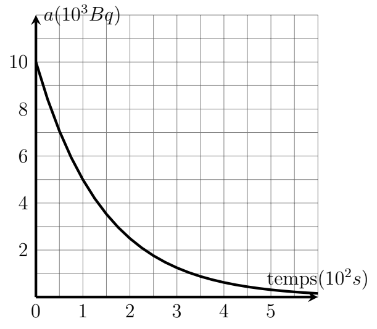
\includegraphics[width=0.42\textwidth]{./img/courbe1.png}
  \end{center}
\end{wrapfigure}
On se propose , à partir du graphe ci-dessous , d’établir la loi de décroissance radioactive d’un nucléide :

\begin{enumerate}
	\item Rappeler la loi de décroissance donnant l’activité d’un radionucléide en fonction du
temps .
\item Graphiquement , déterminer l’activité initiale et la demi-vie $t_{1/2}$
\item Calculer la constante radioactif $\lambda$ en précisant son unité .
\item Graphiquement déterminer la constante du temps $\tau$
\item Quelle est la relation entre $\tau$ et $\lambda$ ? Est-elle vérifiée dans ce cas ?
\end{enumerate}
\end{Box2}


\begin{Box2}{Exercice 4 :Datation d’une nappe phréatique }
Le chlore 36 est crée régulièrement dans la haute atmosphère et se trouve dans l’eau. Ilest radioactif $\beta^-$. Les eaux de surface ont une teneurs en chlore 36 constante malgré sa
radioactivité . Leur contact avec l’atmosphère et les mouvements de l’eau permettent d’en garantir le teneur. 

Les nappes phréatiques d’écoulement lent en sous - sol voient leur teneur en chlore 36 diminuer. 

Ainsi, un forage réalisé dans une tel nappe indique que celle - ci ne
contient plus que $33\%$ de chlore 36 par rapport à une eau courante. La demi-vie du chlore
36 est $t_{1/2} = 3, 0. 10^4ans$.

\begin{enumerate}
	\item Écrire l’équation nucléaire de radioactivité du chlore 36 .

	\item Calculer l’âge de la nappe d’eau trouver par forage .
	\item  Est-il possible d’utiliser le silicium 32 pour réaliser cette datation, sachant que sa
		demi-vie est $t_{1/2} = 6,5.10^2ans$
\end{enumerate}

\end{Box2}
%\vspace{2cm}
\begin{center}
   \Large{ \em{Exercices Supplémentaires}}
\end{center}


%\vspace{-0.7cm}
%%%_________________________Exercice 5 : _________________________Exercice
\begin{Box2}{Exercice 5 :Application de la radioactivité dans la médecine }
La médecine est l'un des principaux domaines dans lequel on trouve l’application pratique de la
radioactivité. on utilise dans ce domaine plusieurs éléments radioactifs pour diagnostiquer et traitées
quelques maladies. Parmi ces éléments, on trouve le Sodium 24 : $_{11}^{24}Na$ qui peut nous aider à contrôler la circulation sanguine dans le corps humain. 

\begin{enumerate}
	\item Le Sodium 24 $_{11}^{24}Na$ se désintègre en magnésium $_{12}^{24}Mg$  
		\begin{enumerate}
			\item écrire l’équation de la désintégration du Sodium 24 en précisant le type de la particule émis.
			\item Calculer la constante radioactive $\lambda$ sachant que la demi-vie du Sodium 24 est : $t_{1/2} = 15h$
		\end{enumerate}
	\item Lors d’un accident routier un blessé a perdu un volume $V_p$ du sang. Pour déterminer ce volume $V_p$ on injecte le blessé à $t_0 =0$ par un volume $V_0 = 5 ml$ de la solution de sodium 24 de concentration molaire   $C_0$=$10^{-3} mol/l$.
		\begin{enumerate}
			\item Calculer $n_1$ le nombre de mole (quantité de la matière) de sodium 24 qui reste dans le sang du
blessé à l’instant $t_1 = 3h$.

on donne : la constante d’Avogadro $N_A = 6,022.10^{23} mol^{-1}.$
\item Le résultat de l’analyse d’un volume $V_2 = 2ml$ prélevé dans le sang du même individu à la
	date $t_1$, donne la quantité de la matière $n_2 =2,1.10^{-9} mol$ du Sodium 24 supposant que le sodium 24 est réparti uniformément dans tout le volume sanguin, déduire le
volume Vp du sang perdu lors de cet accident, sachant que le volume du sang dans le corps
humain est de 5L.
		\end{enumerate}
\end{enumerate}



\end{Box2}


	%Pour mesurer la propagation des ondes sonores dans l’air on réalise le montage expérimental représentant ci-dessous, la distance entre les deux microphones R1 et R2 est d=1,70m. La courbe ci-dessous représente la variation de la tension aux bornes de chaque microphone.

%\underline{Donnée : }La sensibilité horizontale : 1ms/div ; température d’air 25°C ; célérité de la propagation du son dans l’eau $V_{eau}$=$1500m/s$.


	%\begin{center}
		%\vspace{-0.5cm}
	%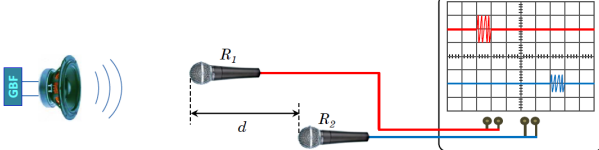
\includegraphics[width=0.7\textwidth]{./img/Ex5.png}
  %\end{center}
%1. Est que le son est une onde longitudinale ou transversale.

%2. Déterminer la valeur du retard temporel entre les microphones R1 et R2.

%3. Déduire la valeur Vair célérité de la propagation des ondes sonores dans l’air.

%4. Déterminer la valeur du retard temporel $\tau'$ quand on déplace le microphone vers la droite à partir de sa position initiale de L= 51cm.

%5. Comparer $V_{air}$ et $V_{eau}$. Que peut-t-on déduire.

%\end{Box2}
%%%_________________________Exercice 6 : _________________________Exercice
%\begin{Box2}{Exercice 6 : échographie}
%\begin{wrapfigure}{r}{0.2\textwidth}
  %\begin{center}
	  %\vspace{-0.6cm}
	%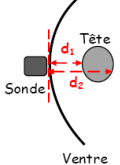
\includegraphics[width=0.2\textwidth]{./img/Exercice6.png}
  %\end{center}
%\end{wrapfigure}
	%Lors d’une échographie d’un foetus, la sonde posée sur le ventre de la mère (voir schéma ci-dessous) émet et reçoit des signaux ultrasonores.

	%L’ordinateur calcule la durée $\Delta{t}$ mis par le signal émis pour faire un aller jusqu’au foetus et un retour jusqu’au récepteur.

%La vitesse v de propagation des ondes ultrasonores dans le corps humain est de $1500 m/s$.

%La sonde orientée vers la tête du foetus reçoit un premier signal avec un décalage
%$\Delta{t}$=$3,0.10^{-5}s$ après l’émission, et un deuxième signal avec $\Delta{t}$=$7,0.10^{-5}s$.

%1. Calculer la distance $d_1$ entre la sonde et la paroi la plus proche de la tête du foetus.

%2. Calculer la distance $d_2$ entre la sonde et la paroi la plus éloigné de la tête du foetus.

%3. Déduire le diamètre d de la tête du foetus en cm.

%\end{Box2}

\end{document}
